\label{sec:justificacion_y_objetivos}

\subsection{Acerca del proyecto}

El presente Trabajo Fin de Grado, parte de un programa ya preexistente que se usa y estudia en la asignatura Tecnologías Multimedia que se llama \textit{Intercom}. El sistema Intercom es una solución de comunicación bidireccional en principio solo de audio pero este trabajo trata y logra solucionar dicho problema implementando, además, la transmisión simultánea de vídeo. Dicho programa permite la transmisión de audio y vídeo en tiempo real simultaneamente. Su diseño se enfoca en la eficiencia y la calidad de la señal asi como, la eficiencia y configuraciones de vídeo posibles pudiendo cambiar tanto la resolución del mismo y su \textit{FPS} (Cuadros por segundo, Frame Rates per Second por sus siglas en inglés). Este sistema está concebido para operar en entornos con limitaciones de ancho de banda y es ejecutable en practicamente cualquier dispositivo por poco potente que sea debido a su eficiencia.
\vspace{\baselineskip}

Dicho programa, \textit{Intercom}, que se encuentra en el repositorio de la asigntuara\footnote{https://github.com/Tecnologias-multimedia/InterCom}, utiliza técnicas avanzadas de procesamiento de señales así como implemnta diversos algoritmos de compresión de datos y optimización de la transmisión de flujos multimedia. 

\vspace{\baselineskip}
Todo el codigo es en el leguaje de programación Python. Ademas, por añadir mas información al contexto en el que se ha realizado este trabajo, esta memmoria ha sido redactada y compuesta en su totalidad en lenguaje LaTex, un sistema de preparación de documentos que permite la creación de documentos de alta calidad tipográfica y es ampliamente utilizado en el ámbito académico y científico. La elección de LaTeX para la redacción de esta memoria no solo garantiza una presentación profesional, sino que también facilita la inclusión de tablas, gráficos y referencias bibliográficas de manera eficiente, personalizada y organizada.

\vspace{\baselineskip}
\begin{center}
	
\includegraphics[width = 0.25\textwidth]{images/LaTeX_logo.png}
	\captionof{figure}{Logo de LaTeX}
	\label{fig:latex}
\end{center}
\vspace{\baselineskip}

\subsection{Justificación y objetivos del proyecto}
La justificación de este proyecto está claramente fundamentado en diversos factores que son altamente relevantes en los tiempos actuales, sobre todo en las áreas académicas, tecnológicas y sociales. Evidentemente, en el mundo tan interconectado en el que vivimos, la comunicación multimedia ha adquirido una importancia crucial en múltiples ámbitos, desde la educación hasta el ámbito profesional y personal. La necesidad de herramientas eficientes y efectivas para la comunicación audiovisual es cada vez más evidente, especialmente en un contexto donde la interacción a distancia se ha vuelto la orden del día.\cite{GSMA}
\vspace{\baselineskip}
\vspace{\baselineskip}
El objetivo principal es facilitar una comunicación clara y fluida, que ya existía en la versión antigua de \textit{InterCom} con el audio, mejorándola con el añadido además, como ya se ha comentado, de la transmisión simultánea de audio y vídeo permitiendo distintas configuraciones de parámetros de vídeo. Evidentemente, se desea lograr este objetivo intentando minimizar la latencia y el uso de recursos de red que es esencial en estos programas de intercomunicación.

\vspace{\baselineskip}
\vspace{\baselineskip}
Entre los objetivos del proyecto estan desarrollar los sistemas necesarios para la captura, transmisión, recepción y visualización del vídeo en tiempo real, garantizando la compatibilidad con el subsistema de audio preexistente además del desarrollo de diversos módulos adicionales para mejorar/adaptar el programa teniendo en cuenta distintas situaciones posibles de ejecución por parte del usuario. Entre ellas, la ejecucion del programa con resoluciones distintas a las permitidas por el dispositivo de la cámara asi, como ajustar los Cuadros por Segundo (\textit{FPS}) deseados por el usuario que sean compatibles con dicha resolución.
\vspace{\baselineskip}


\subsection{Estructura de InterCom}

A continuación, para mayor contexto y comprensión del proyecto, se presenta la estructura jerarquizada de \textit{InterCom} que ilustra la organización de los módulos y componentes del sistema. Esta representación visual proporciona una visión clara de cómo se interrelacionan los diferentes elementos del programa.
\begin{center}
	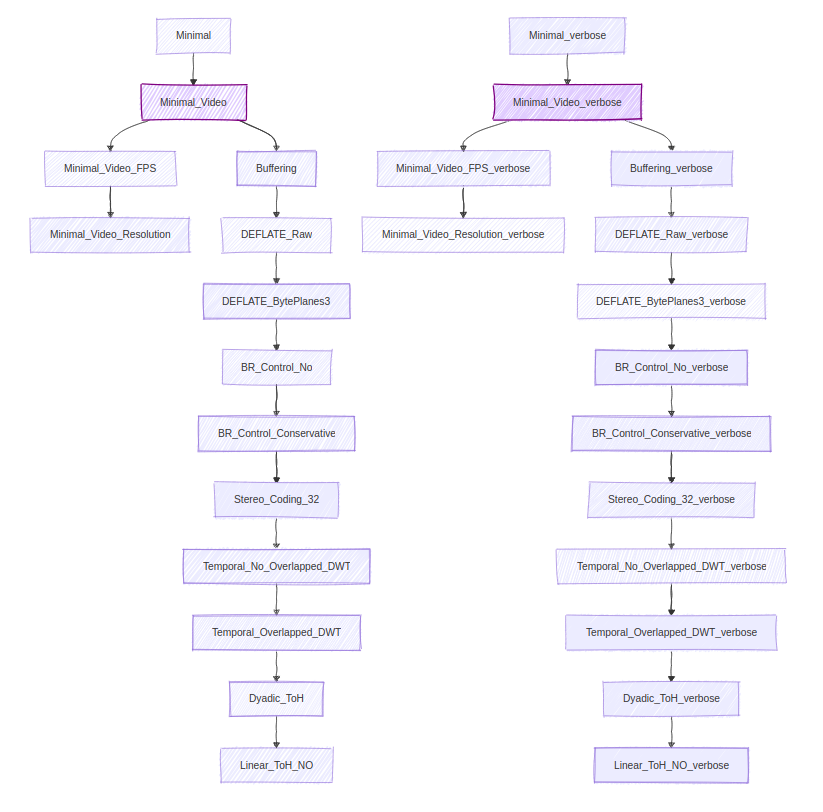
\includegraphics[width = 0.82\textwidth]{images/esquema_jerarquico.png}
	\captionof{figure}{Estructura jeraquizada de InterCom}
	\label{fig:jeraquia}
\end{center}

\vspace{\baselineskip}
Como se puede observar en la figura, el sistema se compone de varios módulos, cada uno de los cuales desempeña un papel específico en la funcionalidad general del programa. El programa base o padre es \textit{Minimal} cuya función es la transmisión sin compresión, sin cuantificación, sin transformación, simplemente una transmisión bidireccional (\textit{full-duplex}) de trozos (\textit{chunks}) sin procesar y que sean reproducibles. De esta, parten todos los demás módulos que componen \textit{InterCom}. 

\vspace{\baselineskip}
En nuestro caso, nos centraremos en el módulo \textit{Minimal Video} y su version \textit{verbose}\footnote{La versión verbose simplemente muestra al ejecutar, estadísticas y datos adicionales a la versión normal} asi como, los módulos \textit{Minimal Video FPS} y \textit{Minimal Video Resolution} y sus versiones \textit{verbose} correspondiente. que son los que se han implementado y desarrollado en este trabajo.

\vspace{\baselineskip}
Como hemos comentado, el módulo \textit{Minimal Video} es el encargado de la transmisión de vídeo y audio en tiempo real. Este módulo se basa en el módulo \textit{Minimal} y añade la funcionalidad de captura, transmisión y recepción de vídeo, permitiendo una comunicación multimedia más completa. La versión \textit{verbose} proporciona información adicional sobre el rendimiento del sistema durante la ejecución. Este será nuestro módulo base para los otros dos módulos adicionalmente implementados y desarrollados en este trabajo (\textit{Minimal Vidoe FPS} y \textit{Minimal Video Resolution}).